%
\documentclass{article}
\usepackage{amsmath,amssymb,bbm,amsthm}
\usepackage{fullpage}
\usepackage{thm-restate,color,xcolor,xspace}
\usepackage{hyperref,cleveref,graphicx}
\usepackage{algorithm,algorithmicx}
\usepackage[noend]{algpseudocode}
\bibliographystyle{alpha}


%%%%% BEGIN Jason's macros %%%%%
%\newcommand{\f}{\displaystyle\frac}
\newcommand{\f}{\frac}
\newcommand{\cd}{\cdot}
\newcommand{\bn}{\binom}
\newcommand{\sr}{\sqrt}
\newcommand{\cds}{\cdots}
\newcommand{\lds}{\ldots}
\newcommand{\vds}{\vdots}
\newcommand{\dds}{\ddots}
\newcommand{\pge}{\succeq}
\newcommand{\ple}{\preceq}
\newcommand{\sm}{\setminus}
\newcommand{\s}{\subseteq}
\newcommand{\su}{\supseteq}

\newcommand{\sumni}{\sum_{n=1}^\infty}
\newcommand{\sumin}{\sum_{i=1}^n}
\newcommand{\bigcupni}{\bigcup_{n=1}^\infty}
\newcommand{\bigcupin}{\bigcup_{i=1}^n}
\newcommand{\bigcapni}{\bigcap_{n=1}^\infty}
\newcommand{\bigcapin}{\bigcap_{i=1}^n}

\newcommand{\BE}{\begin{enumerate}}
\newcommand{\EE}{\end{enumerate}}
\newcommand{\im}{\item}
\newcommand{\BI}{\begin{itemize}}
\newcommand{\EI}{\end{itemize}}
\def\BAL#1\EAL{\begin{align*}#1\end{align*}}
\def\BALN#1\EALN{\begin{align}#1\end{align}}
\def\BG#1\EG{\begin{gather}#1\end{gather}}

\newcommand{\Sum}{\displaystyle\sum\limits}
\newcommand{\Prod}{\displaystyle\prod\limits}
\newcommand{\Int}{\displaystyle\int\limits}
\newcommand{\Lim}{\displaystyle\lim\limits}
\newcommand{\Max}{\displaystyle\max\limits}
\newcommand{\Min}{\displaystyle\min\limits}

\newcommand{\logn}{\log n}

\newcommand{\dx}{\frac d{dx}}
\newcommand{\dy}{\frac d{dy}}
\newcommand{\dz}{\frac d{dz}}
\newcommand{\dt}{\frac d{dt}}

\newcommand{\inv}{^{-1}}

\newcommand{\R}{\mathbb R}
\newcommand{\Z}{\mathbb Z}
\newcommand{\F}{\mathbb F}
\newcommand{\C}{\mathbb C}
\newcommand{\N}{\mathbb N}
\newcommand{\Q}{\mathbb Q}

\newcommand{\eps}{\epsilon}
\newcommand{\e}{\epsilon}
\newcommand{\de}{\delta}
\newcommand{\De}{\Delta}
\newcommand{\la}{\lambda}
\newcommand{\g}{\gamma}
\newcommand{\G}{\Gamma}
\newcommand{\pt}{\partial}
\newcommand{\al}{\alpha}
\newcommand{\be}{\beta}
\newcommand{\om}{\omega}
\newcommand{\Om}{\Omega}
\newcommand{\el}{\ell}
\renewcommand{\th}{\theta}
\newcommand{\Th}{\Theta}
\newcommand{\m}{\mathcal}
\newcommand{\ol}{\overline}

\newcommand{\Ra}{\Rightarrow}

\newcommand{\lf}{\lfloor}
\newcommand{\rf}{\rfloor}
\newcommand{\lc}{\lceil}
\newcommand{\rc}{\rceil}

\newcommand{\E}{\mathbb E}
\newcommand{\Var}{\textup{Var}}
\newcommand{\Cov}{\textup{Cov}}
\newcommand{\1}{\mathbbm 1}
\newcommand{\poly}{\textup{poly}}
\newcommand{\polylog}{\textup{polylog}}
\newcommand{\pl}{\textup{polylog}}
\newcommand{\norm}[1]{\left\lVert#1\right\rVert}
\newcommand{\vol}{\textbf{\textup{vol}}}

\newcommand{\rank}{\textup{rank}}
\newcommand{\spn}{\textup{span}}
\newcommand{\Tr}{\textup{Tr}}

\newcommand{\lp}{\left(}
\newcommand{\rp}{\right)}
\newcommand{\lb}{\left[}
\newcommand{\rb}{\right]}
\newcommand{\lmt}{\left[\begin{matrix}}
\newcommand{\rmt}{\end{matrix}\right]}


\newtheorem{theorem}{Theorem}[section]
\newtheorem{lemma}[theorem]{Lemma}
\newtheorem{definition}[theorem]{Definition}
\newtheorem{corollary}[theorem]{Corollary}
\newtheorem{observation}[theorem]{Observation}
\newtheorem{claim}[theorem]{Claim}
\newtheorem{subclaim}[theorem]{Subclaim}
\newtheorem{fact}[theorem]{Fact}
\newtheorem{assumption}[theorem]{Assumption}

\newcommand{\BT}{\begin{theorem}}
\newcommand{\ET}{\end{theorem}}
\newcommand{\BL}{\begin{lemma}}
\newcommand{\EL}{\end{lemma}}
\newcommand{\BD}{\begin{definition}}
\newcommand{\ED}{\end{definition}}
\newcommand{\BC}{\begin{corollary}}
\newcommand{\EC}{\end{corollary}}
\newcommand{\BO}{\begin{observation}}
\newcommand{\EO}{\end{observation}}
\newcommand{\BCL}{\begin{claim}}
\newcommand{\ECL}{\end{claim}}
\newcommand{\BSCL}{\begin{subclaim}}
\newcommand{\ESCL}{\end{subclaim}}
\newcommand{\BF}{\begin{fact}}
\newcommand{\EF}{\end{fact}}
\newcommand{\BA}{\begin{assumption}}
\newcommand{\EA}{\end{assumption}}
\newcommand{\BP}{\begin{proof}}
\newcommand{\EP}{\end{proof}}
\newcommand{\BSP}{\begin{subproof}}
\newcommand{\ESP}{\end{subproof}}
\newcommand{\BPS}{\begin{proof}[Proof (Sketch)]}
\newcommand{\EPS}{\end{proof}}
\Crefname{observation}{Observation}{Observations}
\Crefname{claim}{Claim}{Claims}
\Crefname{subclaim}{Subclaim}{Subclaims}
\Crefname{fact}{Fact}{Facts}
\Crefname{assumption}{Assumption}{Assumptions}

\newenvironment{subproof}[1][\proofname]{%
  \renewcommand{\qedsymbol}{$\diamond$}%
  \begin{proof}[#1]%
}{%
  \end{proof}%
}

\newcommand{\alert}{\textcolor{red}}
\newcommand{\para}{\paragraph}
%\newcommand{\defn}{\textbf}

\newcommand{\tO}{\tilde{O}}

\newcommand{\thml}[1]{\label{thm:#1}}
\newcommand{\thm}[1]{\Cref{thm:#1}}
\newcommand{\leml}[1]{\label{lem:#1}}
\newcommand{\lem}[1]{\Cref{lem:#1}}
\newcommand{\defnl}[1]{\label{def:#1}}
\newcommand{\defn}[1]{\Cref{def:#1}}
\newcommand{\clml}[1]{\label{clm:#1}}
\newcommand{\clm}[1]{\Cref{clm:#1}}
\newcommand{\corl}[1]{\label{cor:#1}}
\newcommand{\cor}[1]{\Cref{cor:#1}}
\newcommand{\obsl}[1]{\label{obs:#1}}
\newcommand{\obs}[1]{\Cref{obs:#1}}
\newcommand{\eqnl}[1]{\label{eq:#1}}
\newcommand{\eqn}[1]{(\ref{eq:#1})}
\newcommand{\linel}[1]{\label{line:#1}}
\renewcommand{\line}[1]{line~\ref{line:#1}}
\newcommand{\secl}[1]{\label{sec:#1}}
\renewcommand{\sec}[1]{\Cref{sec:#1}}
%%%%% END Jason's macros %%%%%

\makeatletter
\newcounter{algocounter}
\@ifpackageloaded{hyperref}%
  {\newcommand{\mylabel}[2]% #1=name, #2 = contents
    {\refstepcounter{algocounter}\protected@write\@auxout{}{\string\newlabel{#1}{{\textcolor{black}{\textup{#2}}}{\thepage}%
      {\@currentlabelname}{\@currentHref}{}}}}}%
\makeatother

\renewcommand{\emph}[1]{\textbf{\textup{#1}}}

\newcommand{\mincut}{\textsf{\textup{mincut}}}
\newcommand{\Rsmall}{R_\textup{small}}
\newcommand{\sma}{{\textup{small}}}
\newcommand{\lar}{{\textup{large}}}

\newcommand{\ssc}{{\sc SSMC}\xspace}
\newcommand{\apc}{{\sc APMC}\xspace}
\newcommand{\ct}{{\sc CT}\xspace}


\begin{document}

\title{Reduction from GHTree to SSMC}
\date{\today}
\maketitle

\BD[SSMC Verification]
The input to SSMC Verification is a graph $G=(V,E)$, a source $s\in V$, and values $\tilde\la_v:v\in V\sm\{s\}$ such that $\tilde\la_v\ge\mincut(s,v)$. The task is to determine, for each vertex $v\in V\sm\{s\}$, whether or not $\tilde\la_v=\mincut(s,v)$.
\ED

\BT
There is an algorithm that makes calls to SSMC Verification on graphs with a total of $O(n\log^3n)$ vertices and $O(m\log^3n)$ edges, and runs for max-flow time outside of these calls.
\ET


\begin{algorithm}
\mylabel{step}{\textsc{GHTreeStep}}\caption{\ref{step}$(G=(V,E),s,U)$} 
\begin{algorithmic}[1]
\State Initialize $R^0\gets U$ and $D\gets\emptyset$
\For{$i$ from $0$ to $\lf\lg|U|\rf$}
 \State Compute \alert{minimal} minimum isolating cuts $\{S^i_v:v\in R^i\}$ on inputs $G$ and $R^i$ \linel{Sv}
 \State Call SSMC Verification on graph $G$, source $s$, and values $\tilde\la_v=w(\pt S^i_v)$ for $v\in R^i$. (We do not care about any $v\notin R^i$, so we can set $\tilde\la_v=\infty$ for them.)
 \State Let $D^i\s R^i$ be the union of $S^i_v\cap U$ over all $v\in R^i\sm\{s\}$ satisfying $\tilde\la_v=\mincut(s,v)$ and $|S^i_v\cap U|\le|U|/2$\linel{D}
 \State $R^{i+1}\gets$ subsample of $R^i$ where each vertex in $R^i\sm \{s\}$ is sampled independently with probability $1/2$, and $s$ is sampled with probability $1$
\EndFor
%\State $D\gets D^0\cup D^1\cup \cds\cup D^{\lf\lg|U|\rf}$
\State\Return the largest set $D^i$ and the corresponding sets $S^i_v$ over all $v\in R^i\sm\{s\}$ satisfying the conditions in \line{D} %$D^0\cup D^1\cup \cds\cup D^{\lf\lg|U|\rf}$
\end{algorithmic}
\end{algorithm}

Let $D=D^0\cup D^1\cup \cds\cup D^{\lf\lg|U|\rf}$ be the union of the sets $D^i$ as defined in the algorithm. Let $D^*$ be all vertices $v\in U\sm \{s\}$ for which there exists an $(s,v)$-mincut whose $v$ side has at most $|U|/2$ vertices in $U$. 

\BL\leml{step}
 $\E[|D\cap D^*|] = \Om(|D^*|/\log|U|)$. 
\EL
\BP
%We first prove that $D\s D^*$. Each vertex $u\in D$ belongs to some $S^i_v$ satisfying $w(\pt S^i_v)\le W$. %and $S^i_v\cap U=\{v\}$ for some $v\in U\sm\{s\}$. 
%In particular, $\pt S^i_v$ is an $(s,u)$-cut with weight at most $ W$. It follows that the $(s,u)$-mincut also has weight at most $ W$, and therefore, $u\in D$.

%It remains to prove that $\E[|D|]\ge\Om(|D^*|/\log|U|)$. 
Consider a rooted minimal Steiner Gomory-Hu tree $T$ of $G$ on terminals $U$ rooted at $s$, which exists by \thm{rooted}. 
%By definition of the Steiner Gomory-Hu tree, a vertex $v\in U$ is in $D^*$ iff its path to the root $s$ in $T$ has at least one edge of weight at most $ W$. 
For each vertex $v\in U\sm \{s\}$, let $r(v)$ be defined as the child vertex of the lowest weight edge on the path from $v$ to $s$ in $T$. If there are multiple lowest weight edges, choose the one with the maximum depth. %\alert{The lowest weight edge is unique because there is only one $(v,s)$-mincut.}

%\alert{DP: 1. Need to define rooted minimal Steiner Gomory-Hu tree which is used in the para above. 3. Should we talk about breaking ties among multiple lowest weight edges or add a perturbation at the outset and claim that mincuts are unique? This last fact needs a proof since there could be exponential number of $s-t$ mincuts, so just adding an inverse polynomial perturabtion does not immediately imply uniqueness. But, perhaps use the (classic) isolation lemma?} \textcolor{blue}{I had assumed all $s-t$ mincuts unique in a previous write-up. I do think the new version is better since we also obtain better bounds for unweighted graphs which we can't use isolation lemma for. But maybe a note to the reader that assuming all min-cuts are unique could help with a first reading}

For each vertex $v\in D^*$, consider the subtree rooted at $v$, define $U_v$ to be the vertices in the subtree, and define $n_v$ as the number of vertices in the subtree. We say that a vertex $v\in D^*$ is \emph{active} if $v\in R^i$ for $i=\lf\lg n_{r(v)}\rf$. In addition, if $U_{r(v)}\cap R^i=\{v\}$, then we say that $v$ \emph{hits} all of the vertices in $U_{r(v)}$ (including itself); see Figure~\ref{fig:hits}. In particular, in order for $v$ to hit any other vertex, it must be active. For completeness, we say that any vertex in $U\sm D^*$ is not active and does not hit any vertex.

%\alert{The above definitions are fine, but would be easier to read with (a) some intuition behind when you say that a vertex is active and process of hitting other vertices, and (b) a figure illustrating the notation.} 

%\textcolor{blue}{Jason: added a figure.}

\begin{figure}\centering
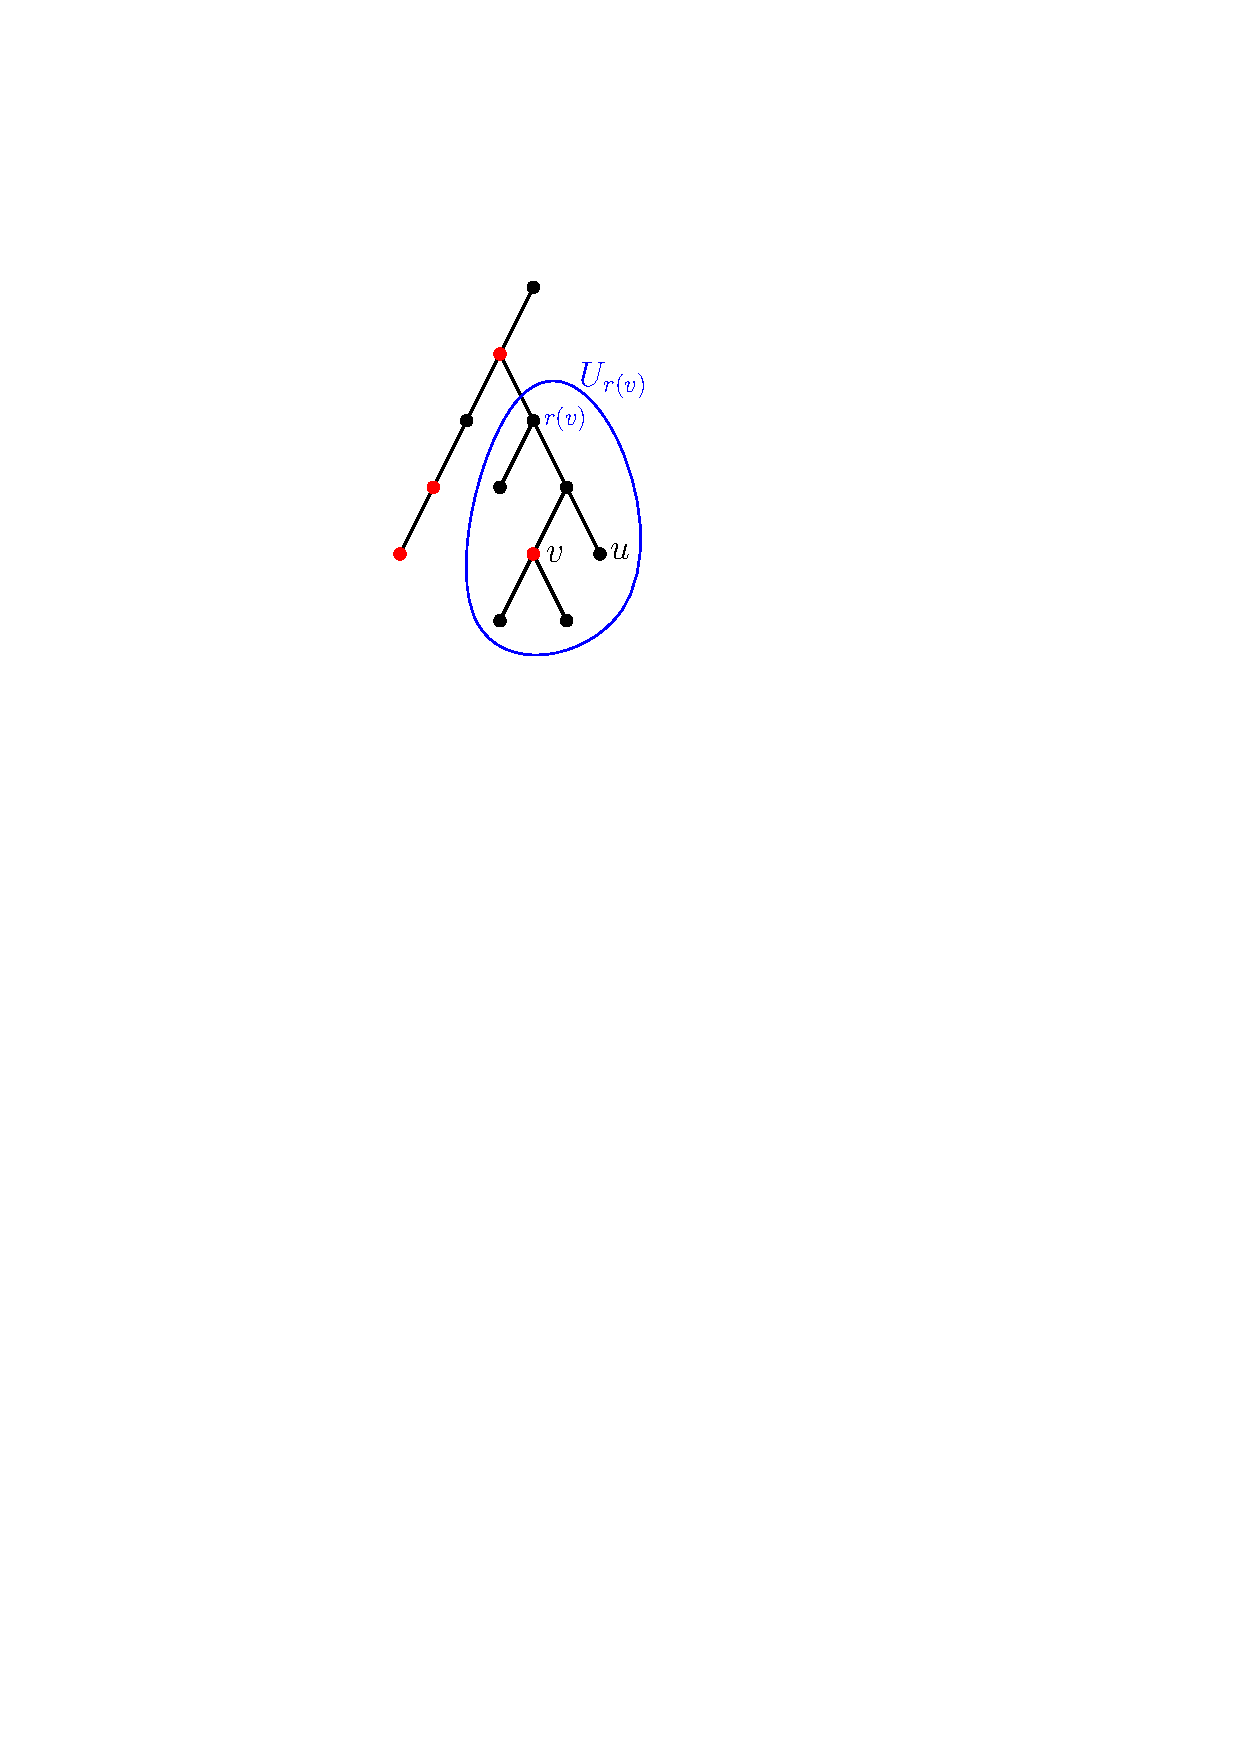
\includegraphics[scale=1]{hits.pdf}
\caption{Let $i=\lf\lg n_{r(v)}\rf=\lf\lg 7\rf=2$, and let the red vertices be those sampled in $R^2$. Vertex $v$ is active and hits $u$ because $v$ is the only vertex in $U_{r(v)}$ that is red.}\label{fig:hits}
\end{figure}

To prove that $\E[|D|] \ge \Om(|D^*|/\log|U|)$, we will show that
 \BE
 \im[(a)] each vertex $u$ that is hit is in $D$, 
 \im[(b)] the total number of pairs $(u,v)$ for which $v\in D^*$ hits $u$ is at least $c |D^*|$ in expectation for some small enough constant $c>0$, and
 \im[(c)] with probability at least $1-\f c{2|U|^2}$ (for the constant $c>0$ in~(b)), each vertex $u$ is hit by at most $O(\log|U|)$ vertices $v\in D^*$. %\alert{DP: There's some play on constants here between the constant hidden in $O(.)$ and the constant in the denominator? Should we make this more explicit?}
 \EE

For (a), consider the path from $u$ to the root $s$ in $T$, and take any vertex $v\in D^*$ on the path that is active (possibly $u$ itself). Such a vertex must exist since $u$ is hit by some vertex. By definition, for $i=\lf\lg n_{r(v)}\rf$, we have $U_{r(v)}\cap R^i=\{v\}$, so $\pt U_{r(v)}$ is a $(v,R^i\sm \{v\})$-cut.  By the definition of $r(v)$, we have that $\pt U_{r(v)}$ is a $(v,s)$-mincut. On the other hand, we have that $\pt f\inv(S^i_v)$ is a $(v,R^i\sm\{v\})$-mincut, so in particular, it is a $(v,s)$-cut. It follows that $\pt f\inv(U_{r(v)})$ and $\pt f\inv(S^i_v)$ are both $(v,s)$-mincuts and $(v,R^i\sm v)$-mincuts, and $\la_v=w(\pt S^i_v)=\mincut(s,v)$. Since $T$ is a minimal Gomory-Hu Steiner tree, we must have $f\inv(U_{r(v)}) \s S^i_v$. Since $S^i_v$ is the minimal $(v,R^i\sm\{v\})$-mincut, it is also the minimal $(v,s)$-mincut, so $S^i_v\s f\inv(U_{r(v)}) $. It follows that $f\inv(U_{r(v)})=S^i_v$. Since $f\inv(U_{r(v)})$ is the minimal $(v,s)$-mincut and $v\in D^*$, we must have $|f\inv(U_{r(v)})\cap U|\le|U|/2$, so in particular, $|S^i_v\cap U|=|f\inv(U_{r(v)})\cap U|\le|U|/2$. Therefore, the vertex $v$ satisfies all the conditions of \line{D}. Moreover, since $u\in U_{r(v)}\s f\inv(U_{r(v)})= S^i_v$, vertex $u$ is added to $D$ in the set $S^i_v\cap U$. \alert{This is the only step that is modified from the original GH-tree paper.}

For (b), for $i=\lf\lg n_{r(v)}\rf$, we have $v\in R^i$ with probability exactly $1/2^i = \Th(1/n_{r(v)})$, and with probability $\Om(1)$, no other vertex in $U_{r(v)}$ joins $R^i$. Therefore, $v$ is active with probability $\Om(1/n_{r(v)})$. Conditioned on $v$ being active, it hits exactly $n_{r(v)}$ many vertices. It follows that $v$ hits $\Om(1)$ vertices in expectation.

For (c), the number of vertices $v$ that hit vertex $u$ is at most the number of active vertices $v$ for which $r(v)$ is on the path from $u$ to $s$ in $T$. Label these vertices $u=v_1,v_2,\lds,v_\el=s$, ordered by increasing distance from $u$ to $r(v_i)$ in $T$. Each vertex $v_j\in D^*$ is active with probability $\Th(1/n_{r(v_j)})$, which is at most $\Th(1/j)$ since $v_1,\lds,v_j \in U_{r(v_j)}$. Each vertex $v_j\notin D^*$ is never active. Therefore, the expected number of active vertices on the path from $u$ to $s$ is at most $\sum_{j=1}^\el\Th(1/j)=\Th(\ln\el)\le \Th(\ln|U|)$. A standard Chernoff bound shows that with probability at least $1-\f c{2|U|^3}$ for any constant $c>0$, the number of active vertices on the path is indeed $O(\ln|U|)$, where the $O(\cd)$ hides the dependency on $c$. Taking a union bound over all $u\in U$, the probability that this is true for all vertices is at least $1-\f c{2|U|^2}$.

Finally, we show why properties (a) to (c) imply $\E[|D|] \ge \Om(|D^*|/\log|U|)$. In the event that property~(c) fails, the total number of pairs $(u,v)$ for which $v$ hits $u$ can be trivially upper bounded by $|U|^2$. Since this occurs with probability at most $\f c{2|U|^2}$, the total contribution to the expectation $c|D^*|$ in property~(b) is at most $c/2$. Therefore, the contribution to the expectation in the event that property~(c) succeeds is at least $c|D^*|-c/2\ge (c/2)|D^*|$. In this case, since each vertex is hit at most $O(\log|U|)$ times, there are at least $\Om(|D^*|/\log|U|)$ vertices hit in expectation.
\EP

\BC\corl{step}
The largest set $D^i$ returned by \ref{step} satisfies $\E[|D^i\cap D^*|] = \Om(|D^*|/\log^2|U|)$.
\EC

\BL[Krauthgamer et al.\ paper]\leml{random-s}
Suppose the source vertex $s\in U$ is chosen uniformly at random. Then, $\E[|D^*|]=\Om(|U|-1)$.
\EL

\begin{algorithm}[H]
\mylabel{ghtree}{\textsc{GHTree}}\caption{\ref{ghtree}$(G=(V,E),U)$} 
\begin{algorithmic}[1]
%\State $\la\gets $ global Steiner mincut of $G$ with terminals $U$ %\Comment{Sparsify if necessary}
\State $s\gets$ uniformly random vertex in $U$
\State Call $\ref{step}(G,s,U)$ to obtain $D^i$ and the sets $S^i_v$ (so that $D^i=\bigcup S^i_v\cap U$)%, and let $R^j$ and $S^j_v:v\in R^j$ ($0\le j\le\lg|U|$) be the intermediate variables in the algorithm\linel{thr}
%\State For each $j\in\{0,1,\lds,\lf\lg|U|\rf\}$, let $R^j_\sma\gets \{ v\in R^j : |S^j_v\cap U|\le|U|/2 \}$  
%\State Let $i\in\{0,1,\lds,\lf\lg|U|\rf\}$ be the iteration maximizing $\big|\bigcup_{v\in R^i_\sma} (S^i_v\cap U)\big|$ \linel{i}

\ \linel{max}
\For{each set $S^i_v$} \Comment{Construct recursive graphs and apply recursion}
 \State Let $G_v$ be the graph $G$ with vertices $V\sm S^i_v$ contracted to a single vertex $x_v$ \Comment{$S^i_v$ are disjoint}
 \State Let $U_v\gets S^i_v\cap U$
 \State If $|U_v|>1$, then recursively set $(T_v,f_v)\gets\ref{ghtree}(G_v,U_v)$
\EndFor
\State Let $G_\lar$ be the graph $G$ with (disjoint) vertex sets $S^i_v$ contracted to single vertices $y_v$ for all $v\in R^i_\sma$
\State Let $U_\lar\gets U\sm D^i$
\State If $|U_v|>1$, then recursively set $(T_\lar,f_\lar)\gets\ref{ghtree}(G_\lar,U_\lar)$

\
\State Combine $(T_\lar,f_\lar)$ and $\{(T_v,f_v):v\in R^i_\sma\}$ into $(T,f)$ according to \ref{combine}%$((T_\lar,f_\lar),\{(T_v,f_v):v\in R^i_\sma)\}$
%\State Construct $T$ by starting with the disjoint union $T_\lar\cup\bigcup_{v\in R^i_\sma}T_v$ and, for each $v\in R^i_\sma$, adding an edge between $f_v(x_v)\in U_v$ and $f_\lar(y_v)\in U_\lar$ of weight $w(\pt_GS^i_v)$ 

%\Comment{Combine Steiner Gomory-Hu trees together} \linel{combine-T}
%\State Construct $f:V\to U$ by $f(v')=f_\lar(v')$ if $v'\in U_\lar$ and $f(v')=f_v(v')$ if $v'\in U_v$ for some $v\in R^i_\sma$\linel{combine-f}
\State\Return $(T,f)$

\end{algorithmic}
\end{algorithm}



\begin{algorithm}[H]
\mylabel{combine}{\textsc{Combine}}\caption{\ref{combine}$((T_\lar,f_\lar),\{(T_v,f_v): v\in R^i_\sma\} )$} 
\begin{algorithmic}[1]
\State Construct $T$ by starting with the disjoint union $T_\lar\cup\bigcup_{v\in R^i_\sma}T_v$ and, for each $v\in R^i_\sma$, adding an edge between $f_v(x_v)\in U_v$ and $f_\lar(y_v)\in U_\lar$ of weight $w(\pt_GS^i_v)$\linel{combine-T}
\State Construct $f:V\to U$ by $f(v')=f_\lar(v')$ if $v'\in U_\lar$ and $f(v')=f_v(v')$ if $v'\in U_v$ for some $v\in R^i_\sma$\linel{combine-f}
\State\Return $(T,f)$
\end{algorithmic}
\end{algorithm}

\BL[Correctness]
The algorithm \ref{ghtree} returns a Gomory-Hu tree.
\EL
\BP
Basically follows from the proof of Lemma 3.3 in previous GH-tree paper, setting $\e=0$
\EP

\BL[Running time]
W.h.p., the algorithm \ref{ghtree} has maximum recursion depth $O(\log^3n)$.
\EL
\BP
By construction, each recursive instance $(G_v,U_v)$ has $|U_v|\le|U|/2$. By \cor{step} and \lem{random-s}, over the randomness of $s$ and \ref{step}, we have
\[ \E[D^i]\ge \Om(\E[|D^*|]/\log^2|U|) \ge \Om((|U|-1)/\log^2|U|) ,\]
so the recursive instance $(G_\lar,U_\lar)$ satisfies $\E[|U_\lar|]\le(1-1/\log^2|U|)\cd(|U|-1)$. Therefore, each recursive branch either has at most half the vertices in $U$, or has at most a $(1-1/\log^2|U|)$ fraction in expectation. It follows that w.h.p., all branches terminate by $O(\log^3n)$ recursive calls.

Since the graph is unweighted, the instances across a given recursion level have a total of $O(n)$ vertices and $O(m)$ edges. \alert{I don't see immediately how to make it work for weighted graphs. But I didn't think about it too much.} W.h.p., the recursion depth is $O(\log^3n)$, so all the recursive instances together have $O(n\log^3n)$ vertices and $O(m\log^3n)$ edges.
\EP

\end{document}

